\chapter{Results}


\section{KNN Results}
The KNN algorithm is simple to execute, but scales poorly with dataset size and image size. Using a dataset of 1291 images, of size 100x100, the largest bottleneck in the procedure is the generation of the squared distance matrix D2, taking 182 minutes (3 hours and 2 minutes) to complete. This was then saved to prevent the need to recalculate it in future. The time taken to calculate the optimal value of K is also proportional to the number of images, taking 379 minutes (6 hours and 19 minutes) when considering all odd values of K up to and including 1291. Plotting these K-values vs the training error obtained for each value is shown in Figure~\ref{fig:k_values}. The time taken to classify a single instance is 0.25m (15s). Testing though the full set of 1291 to obtain the training classification accuracy takes \~1291*0.25 minutes, resulting in a real-world time of 342 minutes (5 hours and 42 minutes). 

\begin{figure}
	\centering
	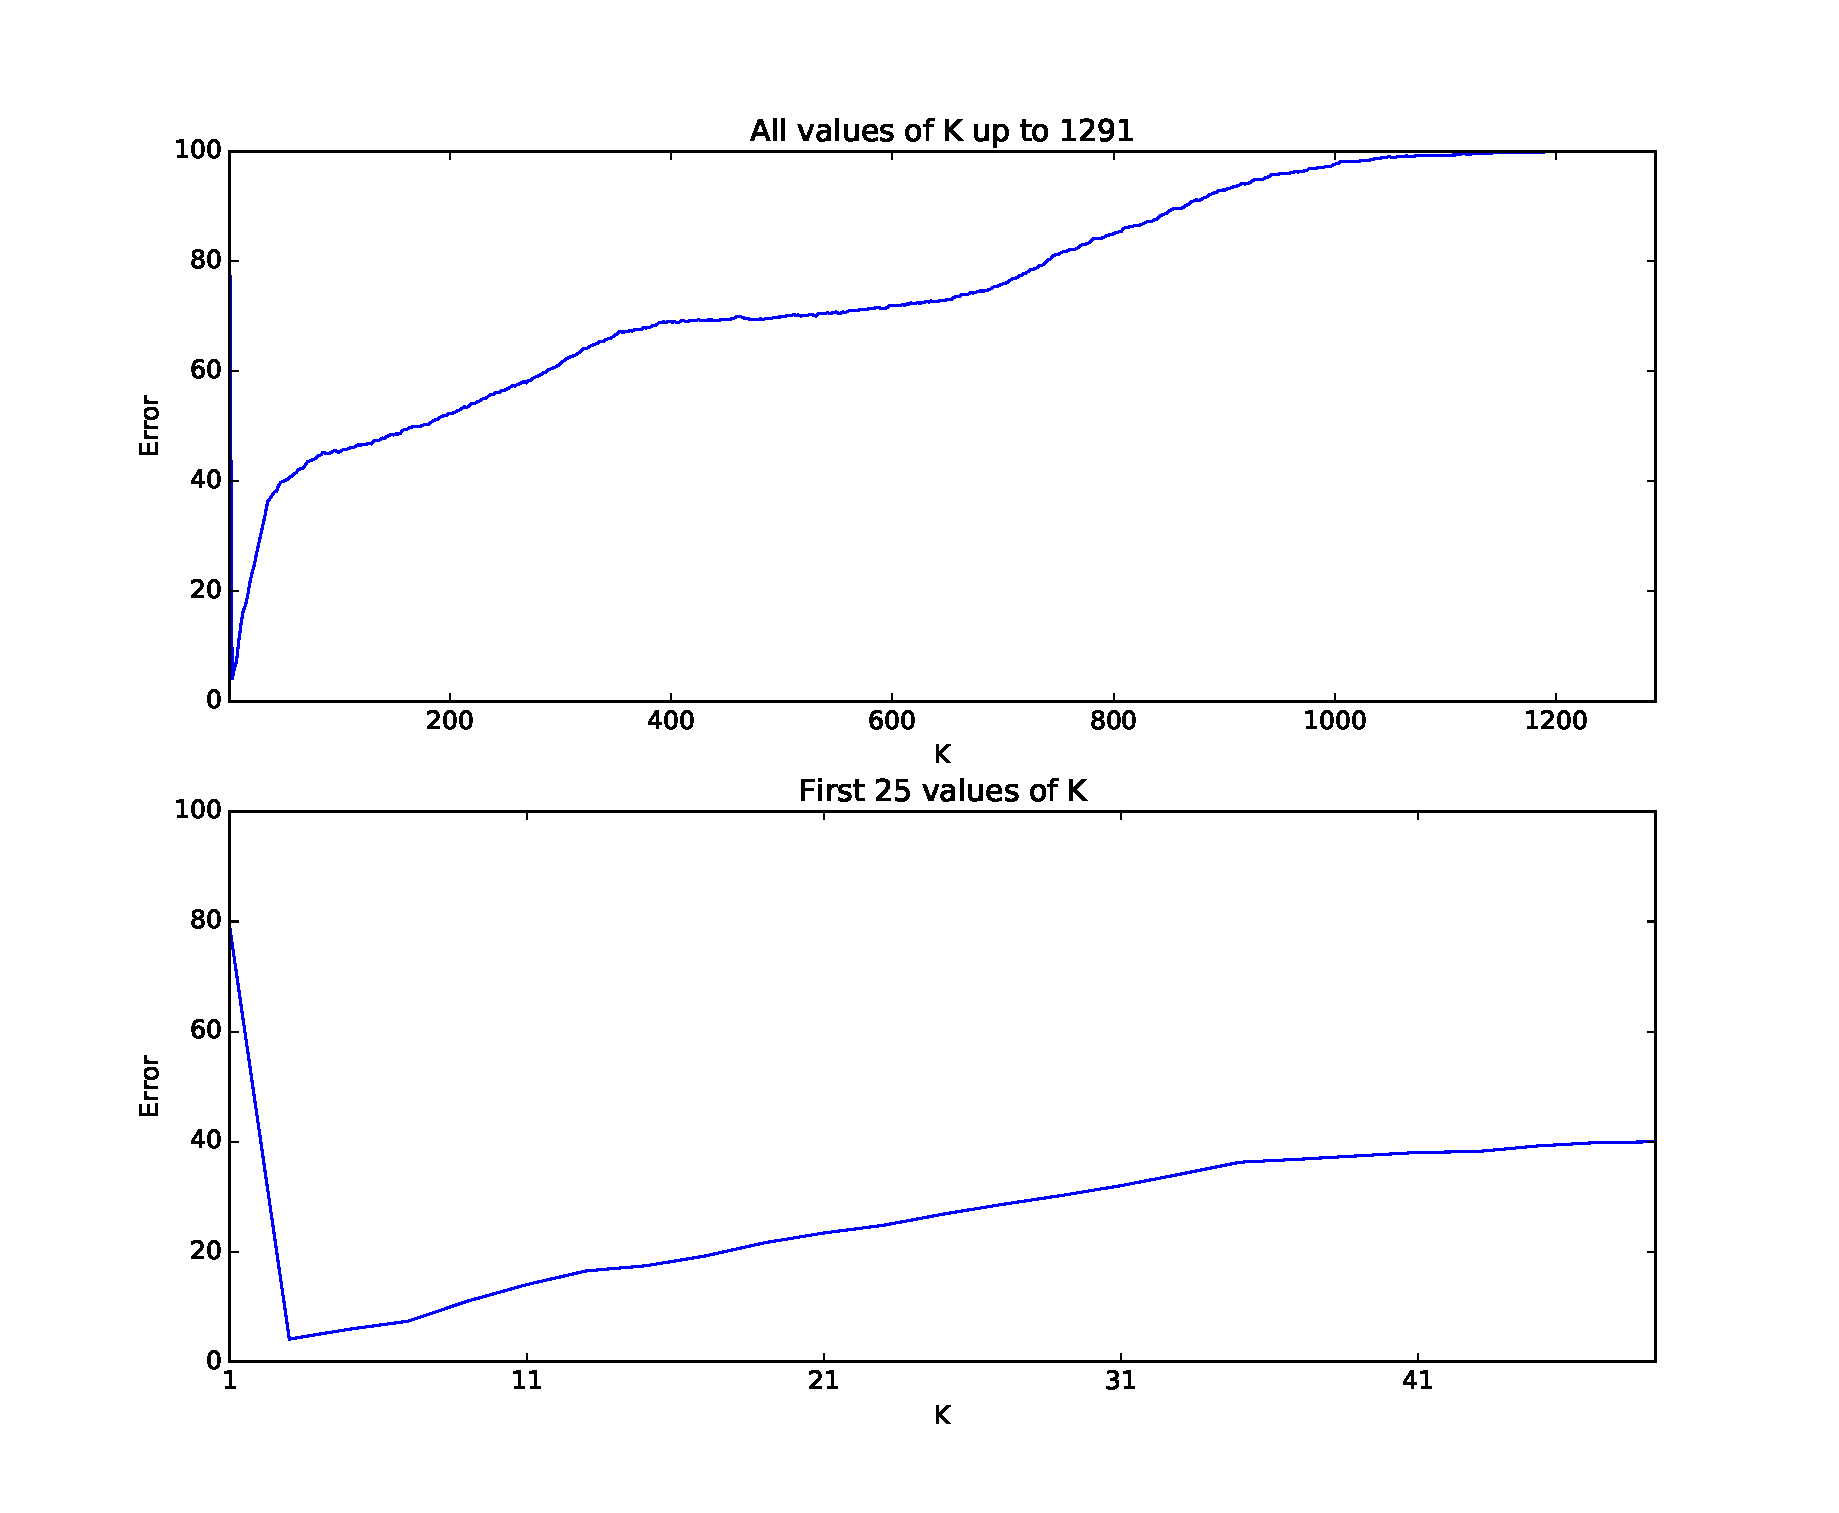
\includegraphics[width=\textwidth]{figures/k_values1291}
	\caption{Optimising for K}
	\label{fig:k_values}
	\centering
\end{figure}


\section{Multilayer Perceptron Initial Results}
The results in this section use an input image of 100x100px. The image is cropped around the center of the image. For some images smaller than this size (e.g. the SLICY set at 54x54px) the images are padded with zeroes to ensure a consistent input image size. The multilayer perceptron has two hidden layers, of 30 and 20 neurons, respectively. The resulting structure is thus 10,000 input neurons feeding into 30, feeding into 20, feeding into the five output neurons. Back-propagation through all layers is applied after every forward run, which has effects on the output that can be seen in ~\ref{sec:analysis}. The cost function is the square of the error. The system is trained for 10,000 iterations, and settles after approximately 300. The input images are taken in order (i.e. 195 BTR 60 images, then 274 2S1 images, etc.) per iteration. The layout of the input data is shown in Table~\ref{tab:input_data}. \\


\begin{table}
	\centering
	\begin{tabular}{|c|c|}
		\hline
		\textbf{Class} & \textbf{No. Images} \\
		\hline
		
		BTR 60 & 195 \\ \hline
		2S1    & 274 \\ \hline
		BRDM 2 & 274 \\ \hline
		D7     & 274 \\ \hline
		SLICY  & 274 \\ \hline
			
	\end{tabular}
	\caption{Input Data}
	\label{tab:input_data}
	\centering
\end{table}

 

\subsection{Analysis}\label{sec:analysis}

The final values of the system lie at 90.6\% classification accuracy (1170/1291 correct). The final confusion matrix (Table~\ref{tab:confusion_fin}) shows a clear pattern; the incorrect predictions are always to the class preceding the correct class. Figure~\ref{fig:avg_cost} shows the average cost decreasing over time, while Figure~\ref{fig:actual_cost} shows how the actual cost sharply increases at the start of a new class and decreases swiftly, before rising again at the beginning of the next class. This appears to be due to the layout of the input data. For subsequent development I need to investigate using batches of inputs to reduce this. Reducing the number of consecutive inputs of the same class should force the network to detect underlying features and mitigate this error.

\subsection{Performance Metrics}



% 440/469   93.8\%
% 689/743   92.7\%
% 932/1017  91.6\%
% 1170/1291 90.6\%

\begin{figure}
	\centering
	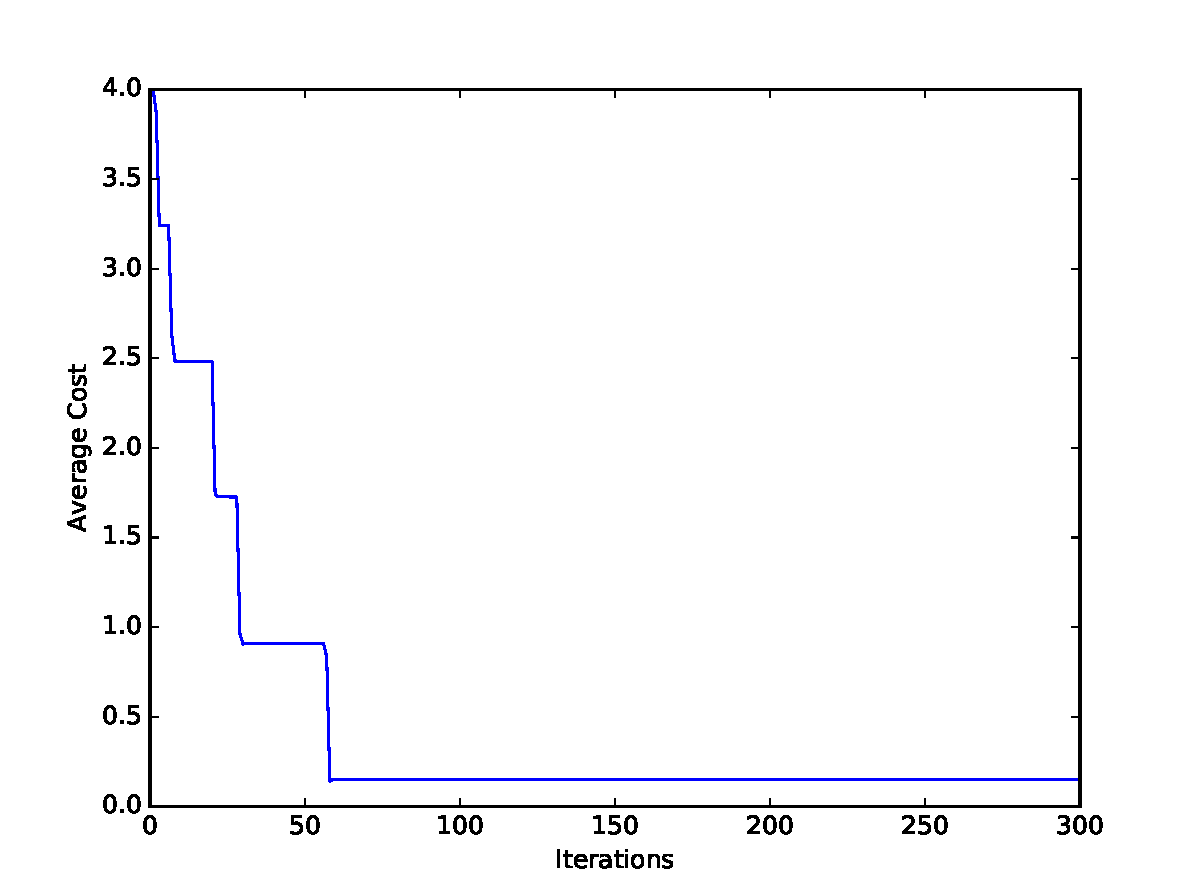
\includegraphics[width=\textwidth]{figures/multilayer_perceptron_average_cost}
	\caption{Average Cost Over Time}
	\label{fig:avg_cost}
	\centering
\end{figure}

\begin{figure}
	\centering
	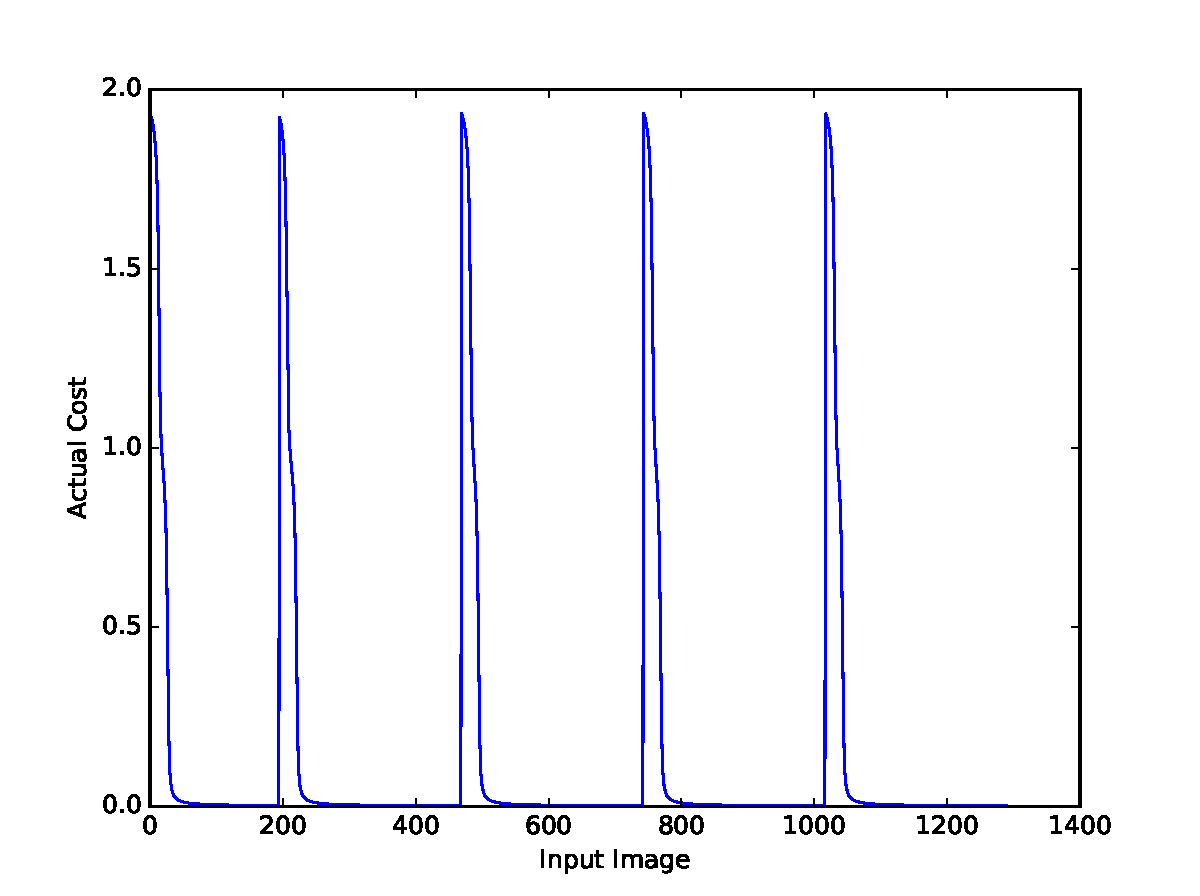
\includegraphics[width=\textwidth]{figures/multilayer_perceptron_actual_cost}
	\caption{Actual Cost Within an Iteration}
	\label{fig:actual_cost}
	\centering
\end{figure}


\begin{table}
	\centering
	\begin{tabular}{|*{7}{c|}}
		
		\cline{3-7}
		\multicolumn{2}{c|}{}         & \multicolumn{5}{|c|}{Predicted Class} 			\\ \cline{3-7}
		\multicolumn{2}{c|}{}                  & BTR 60 & 2S1 & BRDM 2 & D7 & SLICY \\ \hline
		\multirow{5}{*}{\begin{turn}{90}Actual Class\end{turn}}
								      & BTR 60 & 0      & 195 & 0      & 0  & 0 	\\ \cline{2-7}
		                              & 2S1    & 0      & 274 & 0      & 0  & 0 	\\ \cline{2-7}
		                              & BRDM 2 & 0      & 274 & 0      & 0  & 0 	\\ \cline{2-7}
		                              & D7     & 0      & 274 & 0      & 0  & 0 	\\ \cline{2-7}
		                              & SLICY  & 0      & 274 & 0      & 0  & 0 	\\
		\hline
	\end{tabular}
	\label{tab:confusion0}
	\caption{Initial Confusion Matrix (Before Training)}
	\centering
\end{table}

\begin{table}
	\centering
	\begin{tabular}{|*{7}{c|}}
		
		\cline{3-7}
		\multicolumn{2}{c|}{}         & \multicolumn{5}{|c|}{Predicted Class} 			\\ \cline{3-7}
		\multicolumn{2}{c|}{}                  & BTR 60 & 2S1 & BRDM 2 & D7 & SLICY \\ \hline
		\multirow{5}{*}{\begin{turn}{90}Actual Class\end{turn}}
		& BTR 60 & 170    & 0   & 0      & 0  & 25	\\ \cline{2-7}
		& 2S1    & 23     & 251 & 0      & 0  & 0 	\\ \cline{2-7}
		& BRDM 2 & 0      & 24  & 250    & 0  & 0 	\\ \cline{2-7}
		& D7     & 0      & 0   & 24     & 250& 0 	\\ \cline{2-7}
		& SLICY  & 0      & 0   & 0      & 24 & 250 \\
		\hline
	\end{tabular}
	\label{tab:confusion_mid}
	\caption{Transitional Confusion Matrix (Before Final)}
	\centering
\end{table}

\begin{table}
	\centering
	\begin{tabular}{|*{7}{c|}}
		
		\cline{3-7}
		\multicolumn{2}{c|}{}         & \multicolumn{5}{|c|}{Predicted Class} 			\\ \cline{3-7}
		\multicolumn{2}{c|}{}                  & BTR 60 & 2S1 & BRDM 2 & D7 & SLICY \\ \hline
		\multirow{5}{*}{\begin{turn}{90}Actual Class\end{turn}}
		& BTR 60 & 170    & 0   & 0      & 0  & 25	\\ \cline{2-7}
		& 2S1    & 24     & 250 & 0      & 0  & 0 	\\ \cline{2-7}
		& BRDM 2 & 0      & 24  & 250    & 0  & 0 	\\ \cline{2-7}
		& D7     & 0      & 0   & 24     & 250& 0 	\\ \cline{2-7}
		& SLICY  & 0      & 0   & 0      & 24 & 250 \\
		\hline
	\end{tabular}
	\label{tab:confusion_fin}
	\caption{Final Confusion Matrix}
	\centering
\end{table}

